\section{Motivation and Observation}
\label{sec:observation}

\begin{figure}
	\centering
	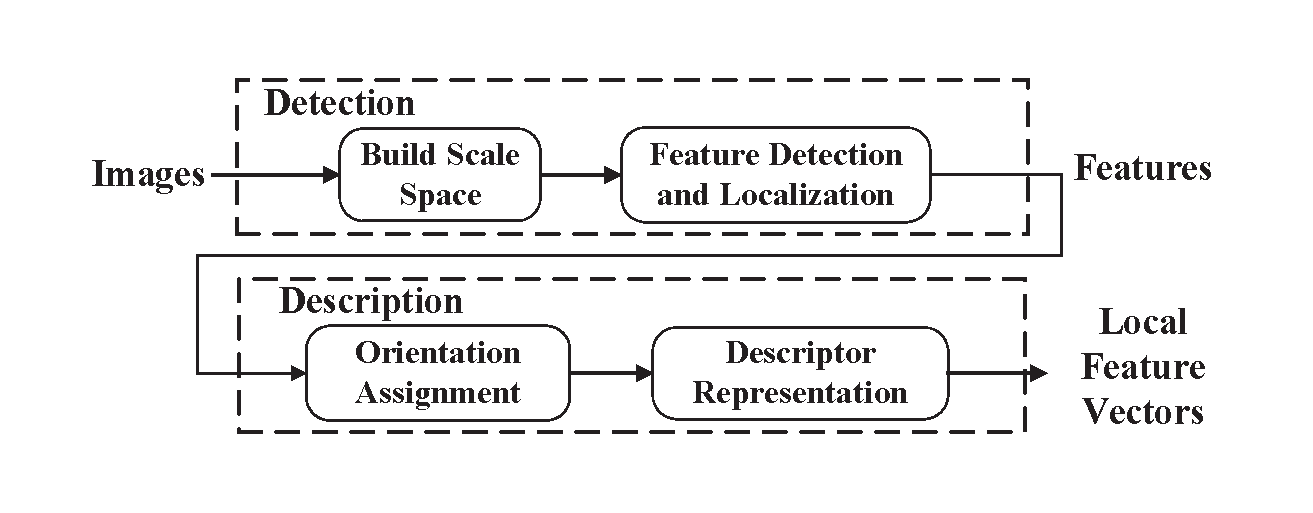
\includegraphics[width=3.5in]{images/fig-workflow.eps}
	\caption{Process flow of a typical local feature descriptor.}
	\label{fig:workflow}
\end{figure}

\begin{figure*}[!t]
	\centering
	\subfigure[Salient region has the densest local features.]{
		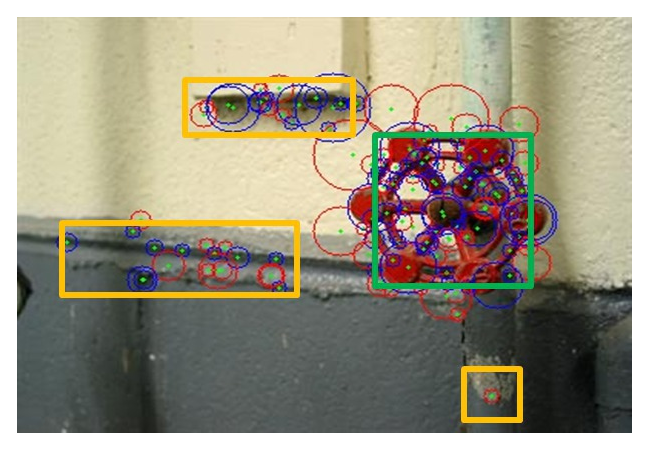
\includegraphics[width=2.2in]{images/fig-observation1.eps}
		\label{fig:observation_1}
	}
	\hfil
	\subfigure[Several salient regions in one image.]{
		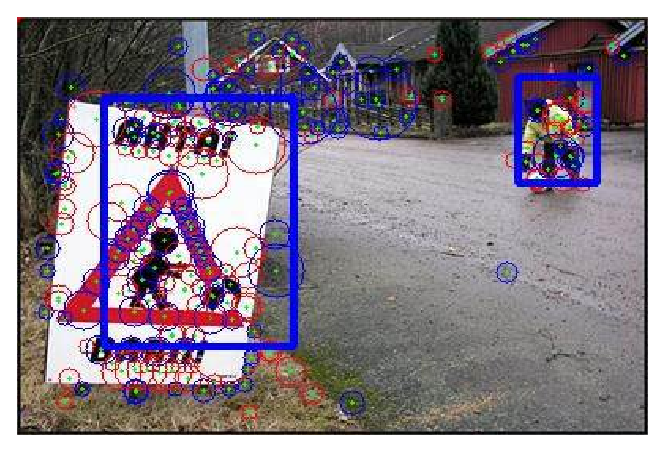
\includegraphics[width=2.2in]{images/fig-observation2.eps}
		\label{fig:observation_2}
	}
	\caption{Example images with local feature based salient regions}
	\label{fig:observations}
\end{figure*}

\subsection{Motivation}

Due to high-accuracy and robustness, {\lfea}s have been widely used in real-world applications. As shown in Figure~\ref{fig:workflow}, they generally consist of two stages: detection and description.  An overview of their processing flow is shown as follows:

\squishlist
\setlength{\itemsep}{0mm}

\item \textbf{Feature Detection:} This stage is to detect \emph{feature points} in an image or a video frame. After an image is initialized, a \emph{m*n} scale space pyramid is constructed to guarantee scale invariant.  After building the scale pyramid, each point in the pyramid is compared with its surrounding 26 points in a 3*3*3 cubic. If its value is the extreme value~(maximum or minimum), the point is chosen as a feature point candidate. To guarantee the quality of extracted points, the candidate points with low contrast or localized along the edges will be discarded. The remaining points are the final feature points.

\item \textbf{Feature Description:} In this stage, each detected point will be described in a high-dimensional vector. First, to make the algorithm rotation invariant, an orientation value is calculated based on the information around it. Then, a descriptor window is constructed and the vector is computed based on the orientation information. The vector value is also normalized to keep the algorithm illumination invariant.
\squishend

There exist two major issues for these local features. First, the processing speed of these local feature algorithms is very slow and among their two stages, description stage is more time-consuming as analyzed in \cite{adaptivepipelineicpp2012}. Second, since they usually extract hundreds of feature points to represent an image and use a multi-dimensionality vector~(64 dimension for SURF and 128 dimension for SIFT) to represent a feature point, the space requirement is also high to store such a great amount of features. To illustrate these two problems, we evaluate the processing time, space requirement, the point number and the proportion of execution time between two stages based on the two most widely used algorithms SIFT and SURF. The hardware is a Core i7 CPU with 4G memory. The dataset is that used in ~\cite{mikolajczyk2005performance}. As the data shown in Table \ref{tab:surfandsift}, it can only finish less than five image processing and the processing time of description stage is at least twice compared to that of the detection stage. Moreover, there are about one thousand points in each image averagely and each image requires about several hundred KB space to storage its feature points.

\begin{table}[!ht]
\begin{center}
\begin{tabular}{|l|c|c|c|c|}
\hline
 & Time(ms) & Space(KB) & Pnum & Proportion \\
\hline
SURF & 171 & 269 & 989   &  1:2\\\hline
SIFT & 719 & 1437 & 2723 & 1:3 \\\hline
\end{tabular}
\end{center}
\caption{Typical time and space consumption of local feature descriptor.}
\label{tab:surfandsift}
\end{table}

As the data shown, for these {\lfea}s, no matter the processing time or the storage space is proportional to the amount of feature points in an image. Therefore, less feature points means  less processing time and less storage space.  Salient region techniques~\cite{cheng2011global,achanta2009frequency,itti1998model} pick up the visual attention parts from an image. Through marking the features outside the region as unimportant and eliminating them, they can be used to reduce the amount of feature points. However, these prior algorithms cannot satisfy the requirements in terms of processing speed and accuracy. The major constraints come from two aspects.
\squishlist
\item \textbf{Limitation of processing speed.} The goal of a salient region algorithm is to detect the visual attention region precisely. Therefore, to provide precise region boundaries, these prior algorithms generally include complex computation, which leads to slow processing speed. In some conditions, their processing speed is even slower than that of {\lfea}, such as SURF. 

\item \textbf{Limitation of accuracy.} In {\lfea}s, a feature point generally is a extreme point in its local region due to its high contrast. Therefore, a lot of local features locate on objects' edges and corners where are also boundaries of salient regions. Since these prior salient region algorithms try to fix the region boundaries precisely, it means the feature points in the boundary cannot be guaranteed to be remained for later retrieval, which would degree the retrieval accuracy. 
\squishend


\subsection{Observation}
\label{subsec:observation}

To overcome these obstacles, we have a comprehensive analysis on the relation between the salient region and the distribution of feature points in images. After studying carefully on the distribution of feature points, we get three major observations:

\begin{description}
	
\item[Observation 1] \desclabel{itm:observation_1} \textit{There exist much denser local features in a salient region.} It means local features we care about locates close to each other, while noisy features or unimportant features are outside and keep a distance away from them. As shown in Figure \ref{fig:observation_1}, local features in the salient region (green box) gather together and many obviously unimportant points locate far away from that box. 

\item[Observation 2] \desclabel{itm:observation_2} \textit{There may exist several salient regions in an image.} In other words, there exists several clusters of local features in an image. For example, the photo in Figure \ref{fig:observation_2} contains two objects, a person and a stop sign, which shape two salient regions following two clusters of local features.

\item[Observation 3] \desclabel{itm:observation_3} \textit{Local features are close to boundaries of salient regions.} From both Figure \ref{fig:observation_1} and Figure \ref{fig:observation_2}, we can find that mostly local features are detected on objects' edges and corners, which are also the boundaries of typical salient regions. 

\end{description}

Observation~\ref{itm:observation_1} indicates that we can detect salient regions directly based on the distribution of local features. In addition, Observation~\ref{itm:observation_2} means it's necessary to deal with the situation of multiple salient regions with multiple clusters of local features in an image. Finally, Observation~\ref{itm:observation_3} shows it's important to avoid eliminating local features on salient regions' boundaries, which require to enlarge actual salient regions to remain these boundary features.